\chapter{Panopto}
\label{ch:panopto}

\begin{preamble}
You have two good tools available for distribution of your lecture
videos: Panopto and YouTube.  Youtube has recently been enabled with your CMU Andrew GSuite account, see Chapter \ref{ch:youtube} for our Youtube guide.
%

We understand that recording and distributing lecture videos can be tedious and time consuming.
%
We have therefore worked on automating some of these tasks in Panopto.  In this
chapter, we describe the Panopto system and some of the automation.
%

%
We have worked with our human resources department so that
administrative assistant can help the faculty with some of these video
recording and distribution tasks, as described throughout this document.
%
We are also piloting more advanced \href{sec:panopto:editing_videos}{video editing} help, provided by admin support staff — but video editing help will be limited to CSD only.
\end{preamble}

\begin{gram}[Introduction]
\label{grm:panopto:introduction}


Panopto is a good mechanism for sharing lecture videos with students.

%It was developed at CMU, in ISR.

Advantages of Panopto include:
	\begin{itemize}
		\item Panopto can be integrated with Zoom: Zoom videos saved to the cloud will upload automatically to your personal Panopto folder. (Section~\ref{sec:panopto:zoom_to_panopto_integration_set_up})
		\item Panopto enables easy and accessible cloud-based video editing. (Section~\ref{sec:panopto:editing_videos})
		\item Panopto enables access control: you can share videos publicly, restrict access to CMU affiliates, restrict access to students, etc. (Section~\ref{sec:panopto:file_transfer_and_access_permissions})
		\item You can assign others (e.g., admin staff, teaching assistants) access to your Panopto folders so that they can assist you with file transfers and releasing videos to students. (Section~\ref{sec:panopto:file_transfer_and_access_permissions})
	\end{itemize}
\end{gram}


	\begin{note}[Help resources]
		This page serves as a guide to get you started with Panopto and to help you utilize the features described above. If you still have questions, please contact the Video Services Team at \href{mailto:coursecast@cs.cmu.edu}{coursecast@cs.cmu.edu}.
	\end{note}


\section{Getting Started}
\label{sec:panopto:getting_started}


\begin{gram}
For faculty, staff, and students:

To gain access to Panopto, email Aaron Caldwell at \href{mailto:aaroncal@andrew.cmu.edu?subject=Creator Access}{aaroncal@andrew.cmu.edu}. Faculty, please also include your course number and course title in this email. Aaron will grant you Creator Access and will assign you a personal folder in which you can upload and save content. Faculty will also be assigned a course folder, where lecture content must be stored once it is ready to be released to students. \textbf{Note: These folders will both initially be \emph{private}, and you will need to adjust access permissions manually, as needed.} Two examples: (1) Professors must assign students access to their course folder so that students can view lectures. (2) Professors may choose to assign their administrative assistants access to their personal and course folders so that their admins can assist with releasing content to students. (See Section~\ref{sec:panopto:file_transfer_and_access_permissions}, ``File Transfer and Access Permissions''.)

After Creator Access has been granted, log in to Panopto at \href{https://scs.hosted.panopto.com/}{https://scs.hosted.panopto.com/} using your Andrew ID and password.
\end{gram}

\section{User Interface}
\label{sec:panopto:user_interface}

\begin{gram}[Browsing the Panopto Video Library]

{
\centering
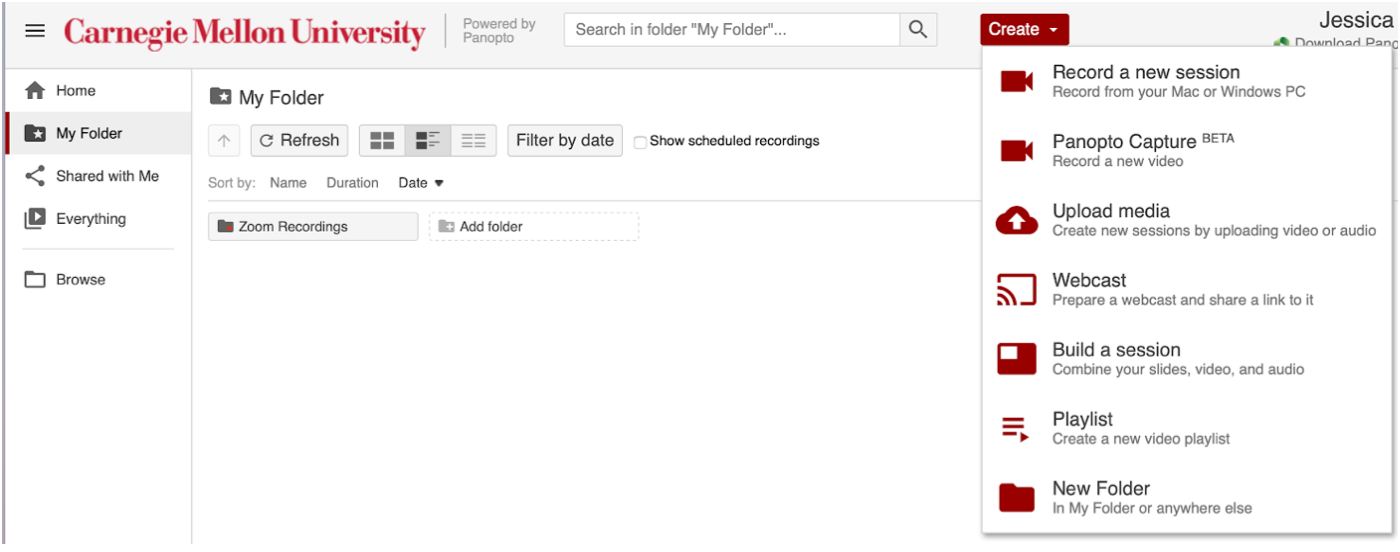
\includegraphics[scale=0.4]{panopto/media/01-ui.png}
}
The 5-minute video below introduces you to Panopto’s user interface and basic features.

	\video{https://scs.hosted.panopto.com/Panopto/Pages/Embed.aspx?id=0f611112-2f7b-4604-8ad6-abc8015c8ace&autoplay=false&offerviewer=true&showtitle=true&showbrand=false&start=0&interactivity=all}{Tour of Video Library}
\end{gram}


\section{Zoom-to-Panopto Integration: Setup}
\label{sec:panopto:zoom_to_panopto_integration_set_up}

Uploading videos and releasing videos to students are time-consuming tasks. To save time, Zoom lectures recorded to the cloud can be configured to automatically upload to Panopto. To enable this integration, follow these two steps:

\begin{gram}[Step 1/2]
	It is important to record your Zoom videos with certain settings enabled. Navigate to \href{https://cmu.zoom.us/}{https://cmu.zoom.us/} and sign in with your Andrew ID and Password. Note that you must use your CMU Zoom account for the integration to work.

	From the left-hand menu, choose ``Settings'' and select the ``Recording'' tab, as shown below.
{
\centering
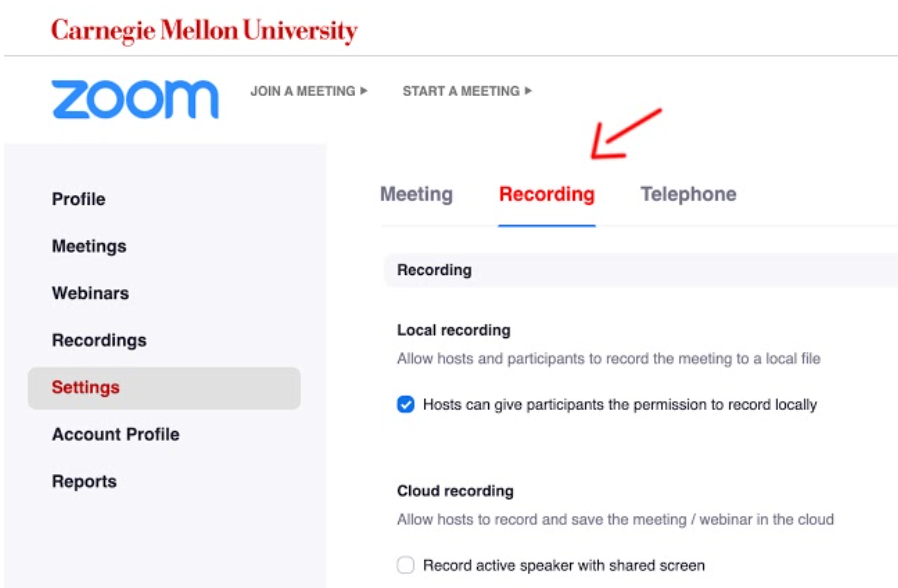
\includegraphics[scale=0.4]{panopto/media/03-recording.png}
}

	The green highlighting in the screenshot below shows the recommended Zoom cloud recording settings for optimal performance. Make sure that your settings match this example.
{
		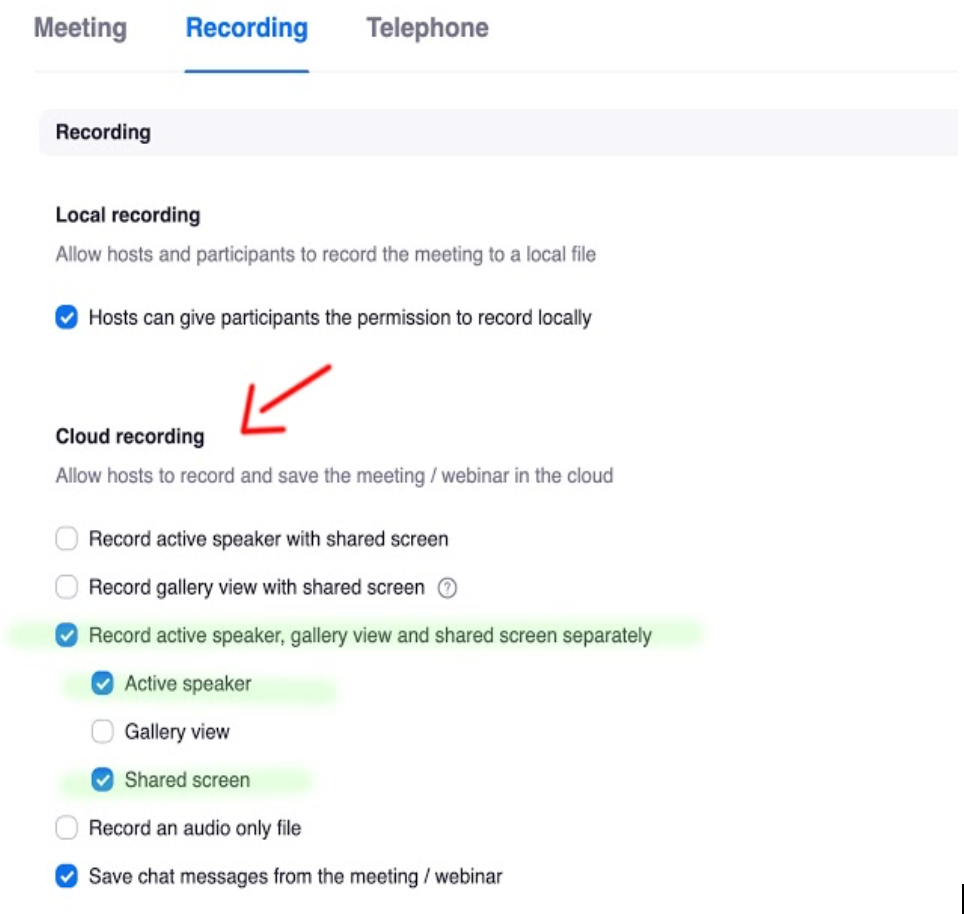
\includegraphics[scale=0.4]{panopto/media/04-settings.png}
}
\end{gram}

\begin{gram}[Step 2/2]
	After you have enabled the settings described above, email Aaron Caldwell at \href{mailto:aaroncal@andrew.cmu.edu?subject=Zoom-to-Panopto}{aaroncal@andrew.cmu.edu} to set up the Zoom-to-Panopto integration. Aaron will let you know when the integration has been enabled.
\end{gram}

\begin{important}[Privacy warning]
	Once the Zoom-to-Panopto integration is enabled, \emph{\textbf{all}} videos recorded to the Zoom cloud will upload to Panopto automatically --- not just your lectures. If you do not want a recording (e.g., a private meeting) to appear on Panopto, then you will need to delete it from Panopto manually after it has uploaded. Zoom meetings that are not configured to record to the Zoom cloud are not affected by this.
\end{important}

\begin{gram}[When the Zoom-to-Panopto Integration is Enabled]
 	At this point, whenever a Zoom cloud recording finishes uploading to Panopto, it will automatically appear in your Panopto ``Zoom Recordings'' folder. Note that this ``Zoom Recordings'' folder is automatically created for you when the Zoom-to-Panopto integration is enabled.
\end{gram}

\begin{gram}[Locating the ``Zoom Recordings'' Folder (1/2)]
	Click on ``My Folder'' in the left-hand menu. Your ``Zoom Recordings'' folder will appear on the subsequent page, as shown in the screenshot below.
{
		\centering
		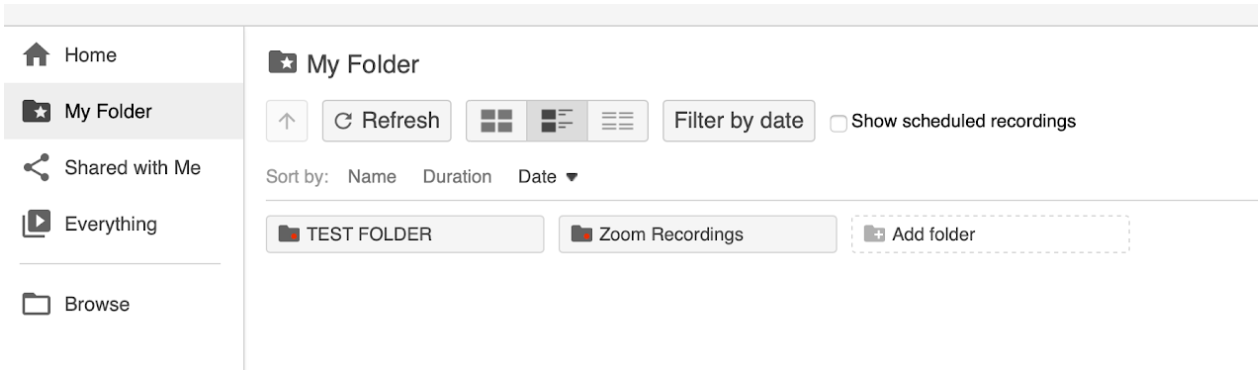
\includegraphics[scale=0.4]{panopto/media/05-my-folder.png}
}
\end{gram}

\begin{gram}[Locating the ``Zoom Recordings'' Folder (2/2)]
	Click on your ``Zoom Recordings'' folder to find your Zoom cloud recordings. The screenshot below shows a Zoom cloud recording that has finished uploading to Panopto.
{
		\centering
		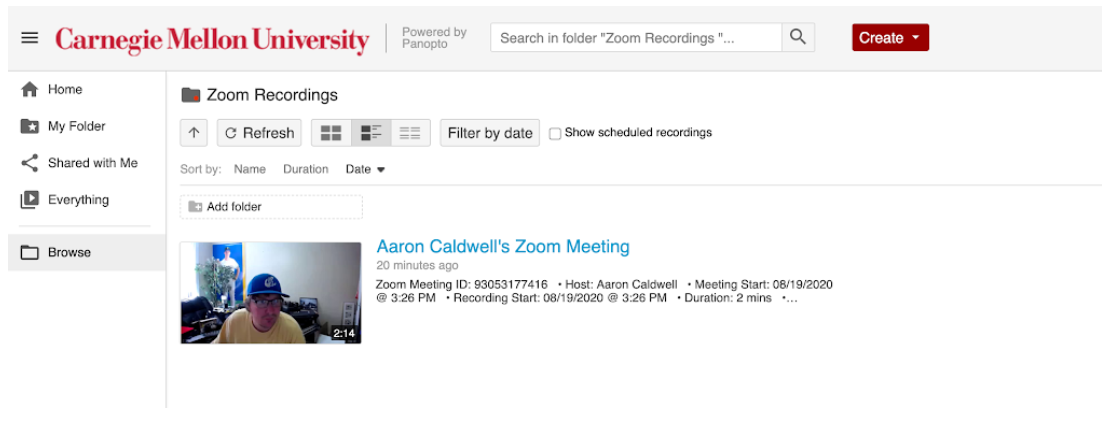
\includegraphics[scale=0.4]{panopto/media/06-zoom-recordings.png}
}
\end{gram}

\begin{gram}[Processing Time]
	Most lecture recordings will take 1-2 hours to appear in Panopto. \textbf{By default, all users assigned access to the ``Zoom Recordings'' folder should receive an email notification when a video has finished populating.} This means that you and your assistant (if your assistant has been assigned access to your ``Zoom Recordings'' folder) will know when a video is able to be released to the students, i.e., when it is ready to be moved to the course folder. Note that this default setting can be adjusted under your ``User Settings''. \textit{If you plan to rely on this feature, please double check under your ``User Settings'' to make sure that you are configured to receive email notifications.}
\end{gram}

\begin{important}[Privacy warning]
	Because \emph{\textbf{all}} Zoom cloud recordings (your lectures, your private meetings, etc. recorded to the Zoom cloud) will upload to your Panopto ``Zoom Recordings'' folder, we advise that you keep this folder private or restrict its access to yourself and your admin only. This means: you or your admin must move the appropriate Zoom recordings \emph{from} your ``Zoom Recordngs'' folder, \emph{to} your Panopto course folder for the recordings to be accessible to your students. Details on this workflow are described in Section~\ref{sec:panopto:file_transfer_and_access_permissions}, ``File Transfer and Access Permissions''. Zoom meetings that are not configured to record to the Zoom cloud are not affected by this.
\end{important}


\section{Manually Uploading Videos}
\label{sec:panopto:manually_uploading_videos}

If you choose not to implement the Zoom-to-Panopto integration, then you must upload locally-saved recordings to Panopto by hand. To do this, click ``Create'' and click ``Upload Media'', as shown below.
{
	\centering
	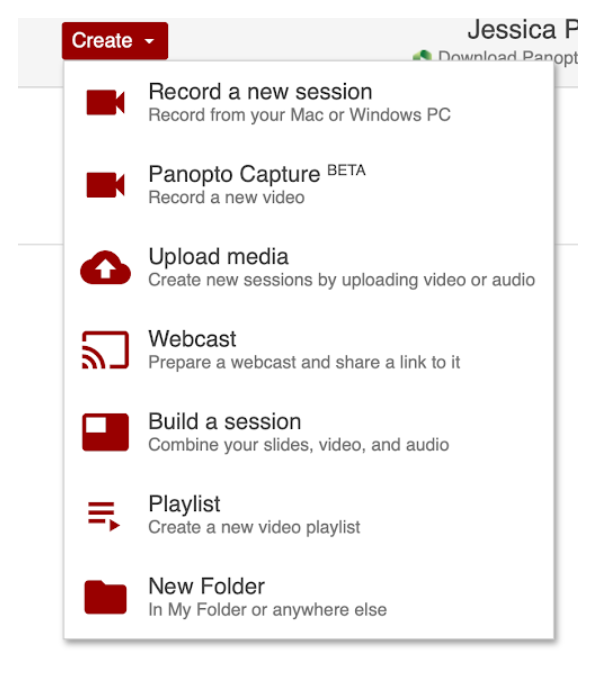
\includegraphics[scale=0.4]{panopto/media/07-create.png}
}


\section{Editing Videos --- Optional Step}
\label{sec:panopto:editing_videos}

Faculty may choose to edit a video before that video is released to students. Panopto enables cloud-based video editing (i.e., no expensive hardware or software is required to edit videos on Panopto). Note that Panopto’s video editor is non-destructive, so there is never any risk of making a mistake and losing video content irrevocably.

Common editing tasks:
\begin{itemize}
	\item Removing ``extra'' time at the beginning and end of a video (e.g., student chatter), or unwanted pauses and interruptions
	\item Adding section titles/transitions
	\item Re-splicing video sections into a new order
\end{itemize}

\begin{gram}[Tutorial]
	Below is a video to help you get started with editing in Panopto.

	\video{https://scs.hosted.panopto.com/Panopto/Pages/Embed.aspx?id=e954eaed-4746-485d-b2c7-abc8015a6977&autoplay=false&offerviewer=true&showtitle=true&showbrand=false&start=0&interactivity=all}{Video Editing Tutorial}

\end{gram}

\begin{note}[Help resources]
If you---a professor, staff member, or student---need help with
editing, please contact
\href{mailto:coursecast@cs.cmu.edu}{coursecast@cs.cmu.edu}. The Video
Services Team can answer questions and, if needed, schedule a meeting
for hands-on instruction.
\end{note}

\section{File Transfer and Access Permissions}
\label{sec:panopto:file_transfer_and_access_permissions}

\begin{gram}[File Transfer]
	When your video has finished uploading to Panopto and is ready to be released to students, you must move your video to the appropriate course folder. Below is a short video that reviews the quick-and-easy steps required to transfer your lecture recording to the appropriate course folder.

	\video{https://scs.hosted.panopto.com/Panopto/Pages/Embed.aspx?id=4ca56daf-b8af-4b5e-adf2-ac1d00261688&autoplay=false&offerviewer=true&showtitle=true&showbrand=false&start=0&interactivity=all}{Lecture Video Folder Transfer Tutorial}
\end{gram}

\begin{important}[Granting students access]
	Remember that once you have been assigned a course folder, this course folder will initially be \emph{private}. You must adjust your course folder access permissions so that course participants (students, teaching assistants, administrative assistants) are able to view lecture content. Various ways to accomplish this are described below.
\end{important}

\begin{gram}[Types of Access Permissions]
	There are various levels of access that you can authorize. Review the possibilities below:

\begin{itemize}
		\item \textbf{Are you using Canvas?} It is possible to integrate Canvas with Panopto. Canvas users who are enrolled in a Canvas course will be asked to authenticate their identities before watching a course video on Panopto. Please contact Aaron Caldwell at \href{mailto:aaroncal@andrew.cmu.edu?subject=Canvas and Panopto}{aaroncal@andrew.cmu.edu} to set up this feature.

		\item \textbf{Are you using Diderot?} You can embed Panopto videos into your Diderot lecture notes or slides by simply using the embed-link for the video. Access control policies that you have specified will apply.

		\item \textbf{Specific people (i.e., restricted access).} Enter a list of specific Andrew IDs, i.e., your students’ IDs. This is a tedious task for large courses that require restricted access but are not on Canvas. To avoid having to enter your students’ IDs manually, contact Aaron Caldwell at \href{mailto:aaroncal@andrew.cmu.edu?subject=Restrict Course Access}{aaroncal@andrew.cmu.edu}. He will create an internal Panopto list of Andrew IDs in order to restrict course access to only course participants. In your email to Aaron, remember to note any teaching or administrative assistants who also require course access.
		\item \textbf{``Anyone at your \emph{organization} with a link.''} Post the link to the video lectures anywhere on the web or distribute the link by email. Anyone with an Andrew ID can navigate to the link and view lecture content.
		\item \textbf{``Anyone with the link.''} Post the link to the video lectures anywhere on the web or distribute the link by email. \emph{Anyone} can view lecture content --- no Andrew ID/authentication required.
		\item \textbf{Public.} The Panopto folder is accessible to anyone on the web. No authentication or link required.
	\end{itemize}
\end{gram}

\begin{gram}[Changing the Access Permissions for a Panopto Folder]
	 Below is a short video that reviews the quick-and-easy steps required to change the access permissions for a given Panopto folder.

	 \video{https://scs.hosted.panopto.com/Panopto/Pages/Embed.aspx?id=78b538c5-b269-4a1d-ba5d-ac1d00eeed08&autoplay=false&offerviewer=true&showtitle=true&showbrand=false&start=0&interactivity=all}{Setting Access Controls Tutorial}
\end{gram}

\begin{note}[Granting your admin/teaching staff access]
	Faculty may choose to give their administrative and/or teaching assistant(s) access to their personal folders (e.g., their ``Zoom Recordings'' folder) so that their admin or TA(s) can assist with releasing content to students. This is useful if the instructor is unavailable when a video has finished uploading to the ``Zoom Recordings'' folder or to another personal folder. Their assistant can release the video (i.e., move the video to the course folder, as described above) on their behalf so that the video is available to students quickly.
\end{note}

\begin{note}[Email notifications]
		Users assigned access to a Panopto folder should receive an email notification when a new video has finished uploading. This setting can be adjusted in ``User Settings''. \textit{If you plan to rely on this feature, please double check your ``User Settings'' to make sure that you are configured to receive email notifications.}
\end{note}
